
\documentclass[twocolumn]{article}
\usepackage{mathpazo}
\usepackage{microtype}
\usepackage{times}
\usepackage{titlesec} % 1
%\usepackage{sectsty} % "제 1 절" ...

 %%%%%%%%%%%%%%%%%%%%%%%%%%%%%%%%%%%%%%%%%%%%%%%%%%%%%%%%%%%%%%%%%%%%%%%%%%%%%
 %                              My Commands
\newcommand{\bi}{\begin{itemize}}
\newcommand{\ei}{\end{itemize}}
\newcommand{\be}{\begin{enumerate}}
\newcommand{\ee}{\end{enumerate}}
\newcommand{\ii}{\item}
\newtheorem{Def}{Definition}
\newtheorem{Lem}{Lemma}
\usepackage{algorithm}
\usepackage{algorithmicx}
\usepackage{algpseudocode}

\usepackage{graphicx}
\graphicspath{%
        {converted_graphics/}
        {./images/}
}

\usepackage{color}
\usepackage{xcolor}
\usepackage{listings}
\usepackage{caption}
\DeclareCaptionFont{white}{\color{white}}
\DeclareCaptionFormat{listing}{\colorbox{gray}{\parbox{\textwidth}{#1#2#3}}}
\captionsetup[lstlisting]{format=listing,labelfont=white,textfont=white}
\usepackage{verbatimbox}

\usepackage[hangul,nonfrench,finemath]{kotex}
    
\setlength\textwidth{7in} 
\setlength\textheight{9.5in} 
\setlength\oddsidemargin{-0.25in} 
\setlength\topmargin{-0.25in} 
\setlength\headheight{0in} 
\setlength\headsep{0in} 
%\setlength\columnsep{5pt}
\sloppy 
 
\begin{document}

\title{
\vspace{-0.5in}\rule{\textwidth}{2pt}
\begin{tabular}{ll}\begin{minipage}{4.75in}\vspace{6px}
\noindent\large {\it KIWI Project}@Data Management Research Section\\
\vspace{-12px}\\
\noindent\LARGE ETRI\qquad  \large Technical Report 14ZS1410-TR-54
\end{minipage}&\begin{minipage}{2in}\vspace{6px}\small
218 Gajeong-ro, Yuseong-gu\\
Daejeon, 305-700, South Korea\\
http:/$\!$/www.etri.re.kr/\\
http:/$\!$/sungsoo.github.com/\quad 
\end{minipage}\end{tabular}
\rule{\textwidth}{2pt}\vspace{0.25in}
\LARGE \bf 빅데이터: 정형 데이터를 위한 분산 저장 시스템 \\
\large Bigtable: A Distributed Storage System for Structured Data
}

\date{}

\author{
{\bf Sung-Soo Kim}\\
\it{sungsoo@etri.re.kr}
}

\maketitle

\begin{abstract}
본 기술문서에서는 구글의 빅테이블 기술을 OSDI 컨퍼런스에 제출한 논문을 중심으로 정리한다.

빅테이블은 수천대 이상의 서버에서 페타(peta) 바이트에 달하는 매우 큰 용량의 데이터를 다루기 위해 디자인된 구조화된 데이터(structured data)를 관리하기 위한 분산 저장 시스템(distributed storage system)이다.
구글의 web indexing, Google Earth, Google Finance와 같은, 많은 구글의 프로젝트들의 데이터가 빅테이블에 저장된다. 
이러한 프로젝트들이 서로 다른 다양한 요구사항들을 빅테이블에 요청하고 있음에도 불구하고, 
빅테이블은 높은 성능과 유연성을 이러한 구글 프로젝트들에 성공적으로 제공하고 있다.
이 논문에서는 빅테이블에서 제공하는 간단한 데이터 모델(simple data model)을 설명하고, 데이터의 레이아웃(layout)과 포맷(format)을 다양하게 제어하는 것, 그리고 빅테이블의 디자인과 구현에 대해 설명하고 있다.
\end{abstract}

\section{Introduction}

%\begin{figure}[!t]
%        \centering
%        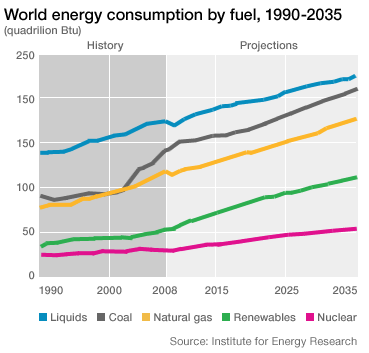
\includegraphics[width=0.33\textwidth]{test}
%        \caption{Caption}
%        \label{fig1}
%\end{figure}
2000년 초부터 구글은 구조화된 데이터(structured data)를 관리하기 위한, 빅테이블이라 불리는 분산 저장 시스템을 디자인하고, 구현하고, 배포했다.
빅테이블은 수천대의 머신(machine)과 페타(peta)바이트의 스케일에서도 신뢰성을 가질 수 있도록 디자인 되었으며, 확장성과 높은 성능, 그리고 유용성등의 목표들을 달성하였다 \cite{Chang:2008:BDS}.

빅테이블은 Google Analytics, Google Finance, Orkut, Personalized Search, Writely, Google Earth 등과 같은 60개 이상의 구글 상품(product) 또는 프로젝트에서 이용이 되고 있으며, 이러한 상품들은 간단한 배치 프로세싱에서부터, 최종 유저에게 잠재되어있는 미묘한 데이터를 제공하는 등과 같은 다양한 요구를 수행하기 위해 빅테이블을 사용한다.
 
 여러가지 관점에서 볼때,  빅테이블은 데이터베이스와 닮았다. 왜냐하면, 빅테이블은 데이터베이스의 구현 전략의 많은 부분을 공유하고 있기 때문이다.
 병렬 데이터베이스(\textit{parallel databases})와 메인 메모리 데이터베이스(\textit{main-memory databases})가 확장성과 높은 처리성능(performance)을 달성했지만, 빅테이블은 그러한 시스템과는 다른 인터페이스를 제공한다. 빅테이블은 관계형 데이터 모델(full relational data model)을 지원하지 않는다. 대신에 데이터 레이아웃과 포맷을 다양하게 컨트롤 할 수 있는 간단한 데이터 모델을 제공한다.
데이터는 임의의 문자열 row와 column 이름들로 인덱싱된다. 사용자가 이러한 데이터를 종종 다양한 형태의 구조화된 데이터로 직렬화(serialize)하려고 할지라도, 빅테이블은 이러한 문자열들을 해석되지 않은 문자열들로 취급해 버린다. 사용자는 데이터를 자신들의 주제에 맞는 선택을 통해 컨트롤 할 수 있다. 결국, 빅테이블의 파라미터들은 사용자가 메모리나 디스크로부터 데이터를 제공받는 것을 다이나믹하게 컨트롤 할 수 있도록 해준다.
 
 %Section 2 에서는 데이터 모델에 대해 더 자세히 설명하고, Section 3 에서는 사용자 API의 개요를 설명한다. Section 4 에서는 빅테이블에 의존하는 구글의 숨겨진 인프라에 대해 설명한다. Section 5 에서는 빅테이블 구현의 기본적인 것들에 대해 설명하고, Section 6 에서는 빅테이블의 성능을 증명하기 위해 만든 것들에 대해 설명한다. Section 7 에서는 빅테이블의 퍼포먼스의 측정에 대한 내용을 제공하며, 빅테이블이 어떻게 구글에서 활용되고 있는지를 Section 8 에서 설명한다. Section 9 에서는 빅테이블을 디자인하고 지원하기 위해 배웠던 것들에 대해 토론한다. 마지막으로, 빅테이블과 관련된 일들을 Section 10 에서 설명하고, Section 11 에서는 우리의 결론을 발표한다.

\section{Data Model}
빅테이블은 산재해 있고(sparse), 분산되어 있으며(distributed), 영구적인 다차원의 잘 정리된 맵(multi-dimensional sorted map)이다. 이 맵은 행 키(row key), 열 키(column key), 타임스탬프(timestamp)로 인덱싱 된다; 맵의 각 밸류(value)는 해석되지 않은 바이트 어레이(bytes array)이다.

{\small \bf
(row:string, column:string, time:int64) → string
}

우리는 빅테이블 같은 시스템을 여러가지 용도의 다양한 방법으로 테스트 해보고나서 이 데이터 모델을 우리의 모델로 확정했다. 우리는 다른 많은 프로젝트에서 웹페이지들의 콜렉션과 관련 정보들이 활용될 수 있다는 가정하에 복사본을 유지하기를 원했으며, 이 특별한 테이블을 웹테이블(Webtable)이라고 부르기로 했다. 웹테이블에서 URL들을 로우 키(row key)로 사용할 것이다. 컬럼 네임(column name) 들로 웹페이지의 다양한 관점들을 저장하고, 콘텐츠(contents)에 웹페이지의 내용을 저장할 것이다. 그림 \ref{fig01} 에서 보이는 것처럼 그 내용이 새로 갱신되었을 때(fetched) 컬럼 아래의 타임스탬프(timestamps)가 생성될 것이다.

\begin{figure}[htb]
        \centering
        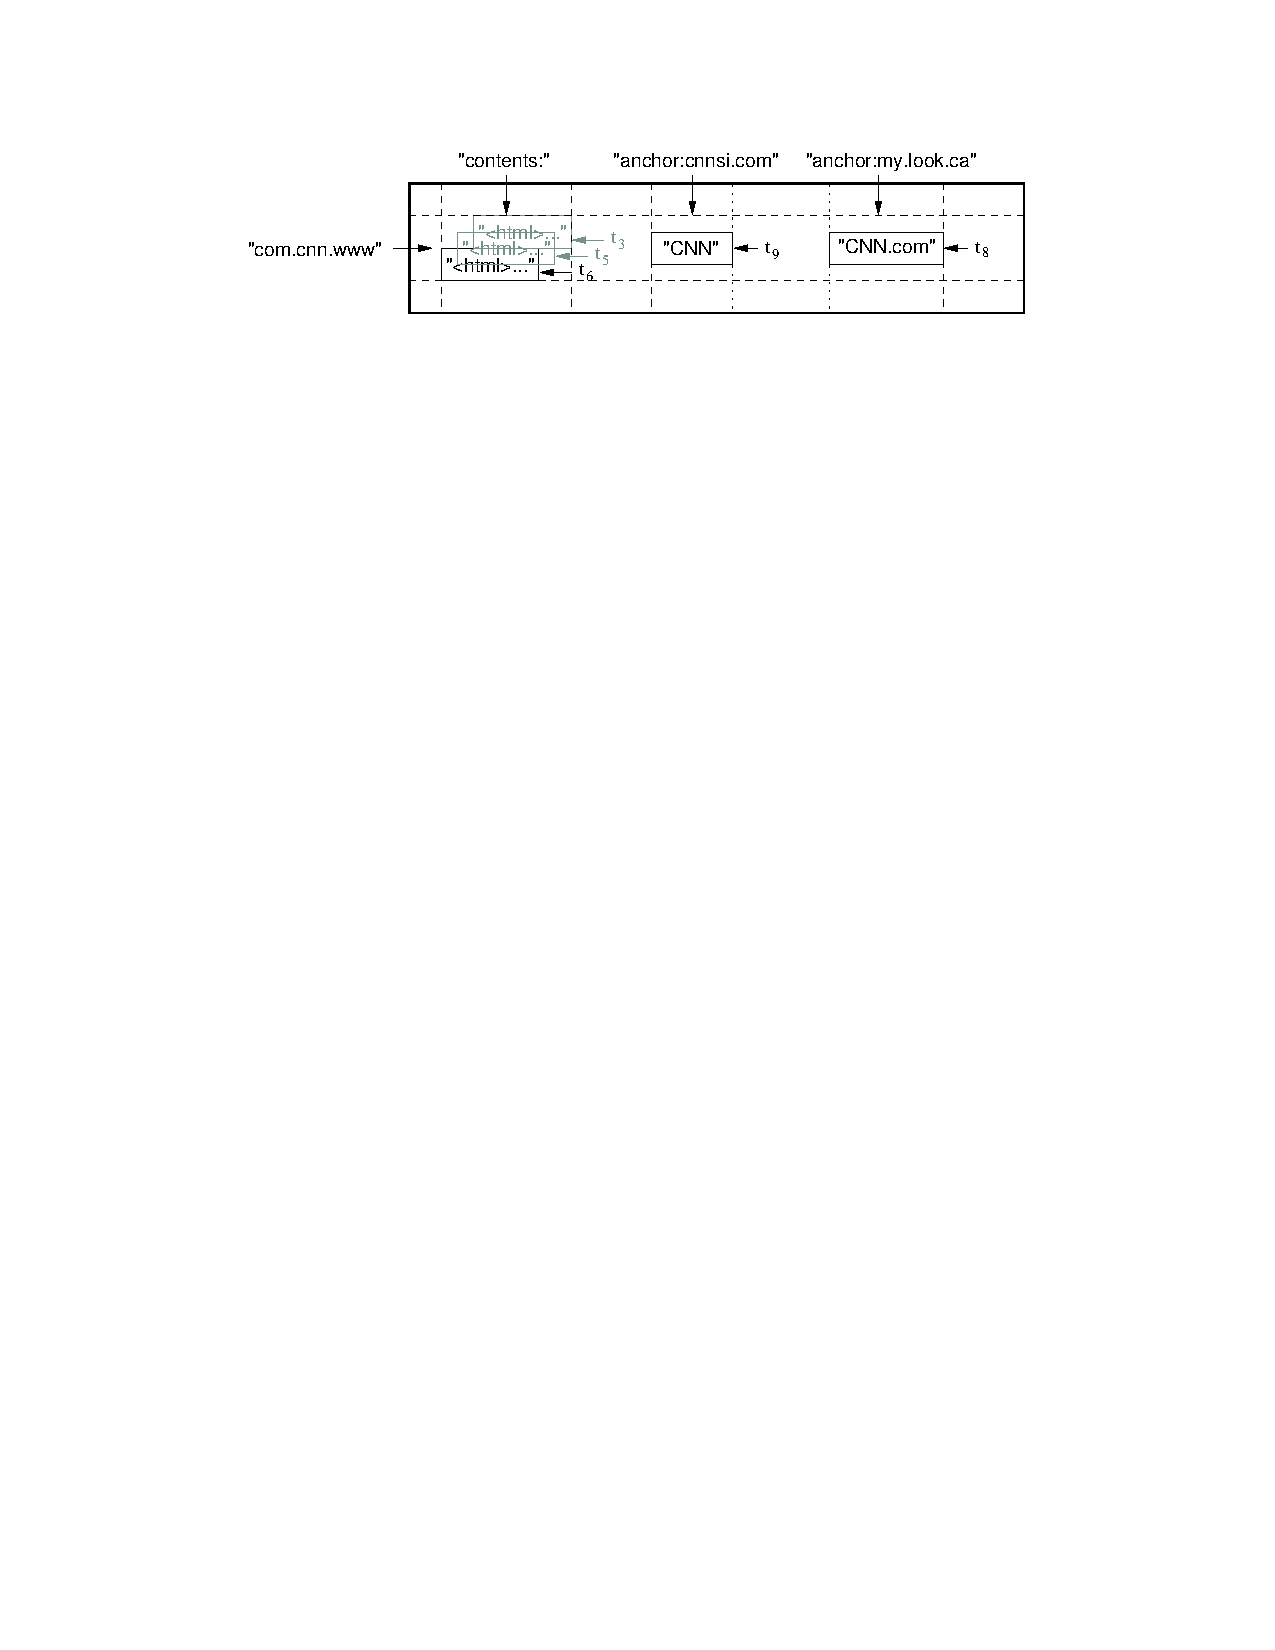
\includegraphics[width=0.48\textwidth]{concept}
        \caption{\small A slice of an example table that stores Web pages. The row name is a reversed URL. The contents column family contains the page contents, and the anchor column family contains the text of any anchors that reference the page. CNN’s home page is referenced by both the Sports Illustrated and the MY-look home pages, so the row contains columns named anchor:cnnsi.com and anchor:my.look.ca. Each anchor cell has one version; the contents column has three versions, at timestamps $t_3$, $t_5$, and $t_6$.}
        \label{fig01}
\end{figure}

 
\subsection*{Rows}
 테이블에서 row key는 최대 64KB의 임의의 문자열이다. (10~100 bytes 가 실제 데이터의 대부분이다.)
하나의 row key는 모든 데이터 읽기와 쓰기의 가장 기본적인 단위이고, 이것은 시스템이 같은 row를 동시에 업데이트 하려는 행동을 보다쉽게 하기 위해 디자인 되었다.
 빅테이블은 row key에 의해 사전을 만드는 것으로 데이터를 유지하고, 만들어진 테이블의 row의 범위는 동적으로 분할된다. 이 분할된 각 row의 범위는 \textit{테이블릿}(\textit{tablet})이라고 부르며, 분산과 로드 밸런싱의 기본 단위가 된다. 결론적으로 짧은 row의 범위가 효율적이며, 적은 수의 머신과 통신만으로 데이터를 읽을 수 있다. 사용자는 자신들의 데이터에 접근하기 위해서 row keys를 선택함으로써 이러한 속성(property)를 활용할 수 있다.
예를들면, 웹테이블에서, 같은 도메인을 사용하는 웹페이지들은 URL의 역순으로 구성된 이름에 의해 연속적인 그룹으로 묶여질 수 있다. 예들들면, 우리는 maps.google.com/index.html 을 com.google.maps/index.html 로 저장한다. 같은 도메인에 있는 페이지들을 근처에 있는 머신에 저장하는 것은 도메인을 분석하는 것을 보다 효율적으로 할 수 있도록 해준다.
 
\subsection*{Column Families}
 Column keys를 그룹화된 집합으로 묶고 이것을 column families라고 부르며, 이것이 접근 제어(access control)의 가장 기본적인 단위의 형태가 된다. 모든 데이터는 column family 안에 저장되고, 대부분은 같은 형태를 갖는다(우리는 같은 column family를 한꺼번에 압축한다). 데이터가 저장되기 전에 반드시 하나의 column family가 생성되며, 그 family 안에는 column key를 가지게 된다.(홍태바리 주석: 그림1에서 보면 anchor:cnnsi.com 과 anchor:my.look.ca는 anchor 라는 하나의 column family이고 그안의 anchor:cnnsi.com 과 anchor:my.look.ca 가 column key 는 column key 이다.)
하나의 테이블안에 분리된 column family의 수를 적게 만드는 것(수백개 정도 안쪽으로..)이 우리의 의도이고, 동작이 일어나는 동안 families 는 거의 변하지 않는다. 그림1에서 보면 웹페이지를 저장하기 위해 생성한 column family는 contents, anchor 둘 뿐이다. 물론 실제로는 더 있을 것이다. 대조적으로, 하나의 테이블안의 column 갯수는 무제한으로 갖게된다.

Column key는 다음과 같은 문법을 갖는다 :
\textit{ family:qualifier}. Column family의 이름들은 반드시 출력이 가능해야(정해져 있어야) 하지만, qualifier는 임의의 문자열이 될 수 있다. 웹테이블에서 하나의 예들들자면 language를 들 수 있다. 여기서 language는 페이지에 씌여진 언어를 말한다. 우리는 language에서 단 하나의 column key만을 사용했고, 각 웹페이지의 언어 ID만을 저장한다. 또다른 column family 예제로 anchor가 있다. 그림1 에서 보는것처럼 anchor family의 column key들은 각각 하나의 anchor를 나타낸다. 참조하는 사이트의 이름이 qualifier이고, 링크 텍스트가 셀안의 내용이 된다.
 메모리 또는 디스크의 접근제어나 계산의 수행은 column family 레벨에서 실행된다. 웹테이블의 예를들면, 어플리케이션에 따라 제어의 형태가 여러가지로 나타난다 : 기본 데이터에 어떤것을 추가하는 경우, 기본 데이터를 읽는 경우, column family를 생성하는 경우, 존재하는 데이터의 열람만 가능하게 하는 경우(또는 열람 조차도 못하게 하는 경우).
 
\subsection*{Timestamps}
 빅테이블의 각 셀은 같은 데이터에 대한 여러개의 버전을 가질 수 있다. 이 버전들은 타임스탬프(timestamps)에 의해 인덱싱된다. 빅테이블의 타임스탬프는 64 비트 정수이다.
 어플리케이션들은 충돌을 피하기 위해서 반드시 유일한 타임스탬프를 생성해야만 한다. 새롭게 생성된 타임스탬프가 셀의 위쪽으로 저장되어 가장 먼저 읽혀질 수 있게 된다. 버전별로 정리된 데이터를 관리하는 것을 편하게하기 위해서, 자동적으로 빅테이블의 가비지 콜렉트를 실행할 수 있는 두가지 세팅을 지원한다. 클라이언트는 가장 최근의 n 개의 버전만을 유지하거나, 새로운 데이터만을 유지할 수 있다(예들들면, 최근 7일간의 데이터 값만 유지하는).
웹테이블의 예를들면, 수집된 페이지의 timestamps를 contents 에 저장되도록 세팅해놨다 : 여기서 페이지는 자동적으로 수집되며, 가비지 콜렉션 메카니즘은 페이지마다 최근 세개의 버전을 유지하도록 되어있다.
 
 
\section{API}
 빅테이블 API는 테이블이나 컬럼 패밀리(column family)를 생성하거나 지울 수 있는 함수들을 제공한다. 또한 클러스터, 테이블, column family, 메타데이타, 접근제어권한과 같은 것들을 변경할 수 있는 함수도 제공한다.
클라이언트 어플리케이션은 빅테이블에 쓰거나 지울 수 있고, 클라이언트 어플리케이션 개인의 row 에서 데이터를 가져오거나, 테이블에 있는 데이터의 하위집합(subset)에 대해서도 이와같은 일을 반복할 수 있다.  아래 코드는 업데이트를 수행하기 위해 RowMutation을 추출하는 C++ 코드를 보여준다. 

\begin{verbnobox}[\scriptsize]
// Open the table
Table *T = OpenOrDie("/bigtable/web/webtable");
// Write a new anchor and delete an old anchor 
RowMutation r1(T, "com.cnn.www");
r1.Set("anchor:www.c-span.org", "CNN"); 
r1.Delete("anchor:www.abc.com");
Operation op;
Apply(&op, &r1);
\end{verbnobox}
 
Apply를 호출함으로 웹테이블에 작은 변경이 일어난다 : www.cnn.com 을 anchor에 더하고 다른걸 지운다.
아래 코드는 특정 row에 있는 모든 anchor들을 반복적으로 추출하는 Scanner를 사용하는 C++ 코드이다. 

\begin{verbnobox}[\scriptsize]
Scanner scanner(T);
ScanStream *stream;
stream = scanner.FetchColumnFamily("anchor"); 
stream->SetReturnAllVersions(); 
scanner.Lookup("com.cnn.www");
for (; !stream->Done(); stream->Next()) {
	printf("%s %s %lld %s\n",
		scanner.RowName(),
          		stream->ColumnName(),
       		stream->MicroTimestamp(),
       		stream->Value());
}
\end{verbnobox}

클라이언트는 다수의 column family에 사용할 수 있고 rows, columns, timestamps 를 검색할 때 사용하는 몇가지 limit 메카니즘을 가지고 있다. 예들들면, 정규표현식 anchor:*.cnn.com 에 매칭되는 것들만 검색하라는 제한을 두거나, 현재시간으로부터 10일 안의 timestamps 만을 가져오도록 할 수 있다.
빅테이블은 더욱 다양한 방법으로 데이터를 조작하기 위해 몇가지 다른 특성들을 지원하고 있다. 첫째로, 빅테이블은 현재 row key간의 일반적인 트랜잭션을 지원하지 않지만 배치(batch)로 row key를 교차하며 기록할 수 있는 기능을 클라이언트 측에 제공한다. 둘째로, 빅테이블은 cell 이 정수 카운터로 사용되는 것을 허락한다. 결국 빅테이블은 서버의 공간에서 클라이언트가 수행할 수 있는 스크립트를 지원한다. 이 스크립트는 Sawzall이라 불리고, 데이터를 처리하기 위해 구글에서 개발한 언어이다. 현재는, Sawzall 을 기반으로한 API 에서 클라이언트의 스크립트가 빅테이블에 데이터를 쓰는 것을 허락하지 않는다. 그러나, 애매한 표현들에 대한 필터링과 다양한 연산자들에 대한 요약을 클라이언트에 제공하고 있다.
 빅테이블은 구글에서 대용량 병렬 처리를 하기위해 개발한 프레임웍인 MapReduce룰 사용할 수 있다. 우리는 빅테이블에서 input source 와 output target 의 경우 모두에 MapReduce job을 사용하기 위해 wrapper를 사용했다.
 
\section{Building Blocks}
빅테이블은 구글의 여러개의 다른 인프라의 조각들로 구성되어 있다. 빅테이블은 로그와 데이터 파일들을 저장하기 위해 분산 구글파일 시스템을 사용한다. 빅테이블은 일반적으로 다양한 분산 어플리케이션들이 실행되는 머신들의 공유된 풀(pool)에서 동작하고, 때로는 다른 어플리케이션들의 프로세스에서 사용하는 머신을 공유하기도 한다. 빅테이블은 job을 스케쥴링하고, 자원을 관리하고, 머신을 공유하고, 머신 오류를 다루고, 머신의 상태를 모니터링하는 부분들을 클러스터 운영 시스템에 의존한다.
 내부적으로 빅테이블의 데이터를 저장하기 위해 구글 SSTable 이라는 파일 포맷을 사용한다. 하나의 SSTable은 key 값들부터 그에 해당하는 value 값들까지 영구적으로 변하지않는 정렬된 맵(ordered immutable map)을 제공하고, 여기에 사용되는 key 값들과 value 값들은 임의의 바이트 문자열이 된다. 구체화된 key 값으로, 관련된 value값을 가져오거나 특정영역의 key/value 쌍을 반복적으로 가져올 수 있는 연산자(operation)들이 제공된다. 내부적으로, 각 SSTable 들은 연속된 블록(blocks)들을 가지고 있다(일반적으로 각 블록은 64KB 이지만 이것은 조절이 가능하다). SStable의 마지막에 저장된 블록 인덱스는 블록의 위치를 찾아내기 위해서 사용된다 : SSTable이 오픈될때 인덱스가 메모리에 올라간다.
단일 디스크 검색으로도 룩업(lookup)이 실행될 수 있다 : 먼저 메모리에 있는 인덱스에서 바이너리 검색을 통하여 적절한 블록을 찾은 다음, 그리고나서 디스크로 부터 적절한 블록을 읽는 것이다. 추가적으로 SSTable을 메모리에 완전히 매핑하고, 디스크 검색을 전혀하지 않는 방법 또한 가능하다.
빅테이블은 Chubby라고 불리는 지속적인 분산 락(lock) 서비스에 의존한다. Chubby 서비스는 다섯개의 활동적인 리플리카(replica)로 구성되어있고, 여기서 하나가 선출되어 마스터가 되고, 들어오는 요청에 능동적으로 반응하게 된다. 리플리카의 과반수 이상이 살아있고, 다른 것들과 통신이 가능할 때 그 서비스는 살아있다고 할 수 있다. Chubby는 리플리카를 지속적으로 유지하고 실패에 대응하기 위해 Paxos 알고리즘을 사용한다. Chubby는 디렉토리들과 작은 파일들로 구성된 네임스페이스를 제공한다. 각각의 디렉토리 또는 파일들은 하나의 락(Lock)으로 사용될 수 있고, 파일에 읽고 쓰는 작업들은 기본적인 작업이 될 수 있다. Chubby 클라이언트 라이브러리는 Chubby 파일의 캐싱(cashing)을 지속적으로 제공한다. 각각의 Chubby 클라이언트들은 하나의 Chubby 서비스에 하나의 session을 갖게되고, session은 session 만료 시간내에 유효 시간을 연장하지 못하면 소멸하게 된다. 클라이언트의 session이 만료되면 모든 락과 열린 핸들을 모두 잃게된다. Chubby 클라이언트는 변경 또는 session의 만료를 알리기 위해서 Chubby 파일과 디렉토리의 콜백(callback)을 등록할 수 있다.
빅테이블은 다양한 용도로 Chubby를 사용한다 : 하나의 활성화된 마스터가 있는지를 보장하는 것과, 빅테이블 데이터의 bootstrap 위치를 저장하는 것, 새로운 타블렛(tablet) 서버를 발견하는 것과 죽은 서버에대한 최종 승인을 하는 것, 빅테이블의 스키마 정보를 저장하는 것, 그리고 접근제어 리스트를 저장하는 것. 만약에 일정기간 동안 Chubby가 이용가능하지 않게된다면, 빅테이블도 이용불가능한 상태가 된다.
 
\section{Implementation}
빅테이블은 세가지 중요한 구성요소로 구현이 된다 : 모든 클라이언트로 연결된 하나의 라이브러리, 하나의 마스터 서버, 그리고 많은 타블렛 서버들.
타블렛 서버들은 부하(workloads)에 따른 적절한 조절을 위해서 클러스터에의해 동적으로 추가되거나 제거가 될 수 있다. 마스터는 타블렛을 타블렛 서버에 할당하거나, 추가되거나 만료된 타블렛 서버를 검출하고, 타블렛 서버의 로드 밸런싱과 구글파일시스템에서의 가비지 콜렉션을 담당하게된다. 게다가, 테이블과 컬럼 패밀리의 생성과 같은 스키마의 변경 또한 핸들링한다. 일반적으로 각각의 타블렛 서버는 서버당 수십에서 수천개의 타블렛을 관리한다. 타블렛 서버는 가지고 있는 타블렛들의 읽기와 쓰기에 대한 요청과, 타블렛의 크기가 너무 커진 경우에 대한 관리를 한다.
대부분의 단일 마스터 분산 저장 시스템에서, 클라이언트 데이터는 마스터를 거쳐서 이동하지 않는다 : 클라이언트는 읽기와 쓰기를 수행하기위해 타블렛 서버와 직접 통신한다. 따라서, 빅테이블 클라이언트는 타블렛 위치 정보를 위해 마스터에 의존하지 않고, 대부분의 클라이언트들은 마스터와 절대 통신하지 않는다. 결론적으로 봤을때, 마스터는 거의 로드가 걸리지 않는다.
빅테이블의 클러스터는 많은 테이블들을 저장한다. 각 테이블은 타블렛의 집합으로 구성되고, 각각의 타블렛은 row range들로 조합된 모든 데이터를 가지고 있다. 테이블의 크기가 커지면, 자동적으로 여러개의 타블렛으로 나눠지고, 대략 그 크기는 100 -- 200MB 정도가 된다.
 
\subsection{Tablet Location}
우리는 타블렛 위치 정보를 저장하기 위해서 B+트리의 그것과 비슷한 3 단계의 계층구조를 사용한다.

\begin{figure}[htb]
        \centering
        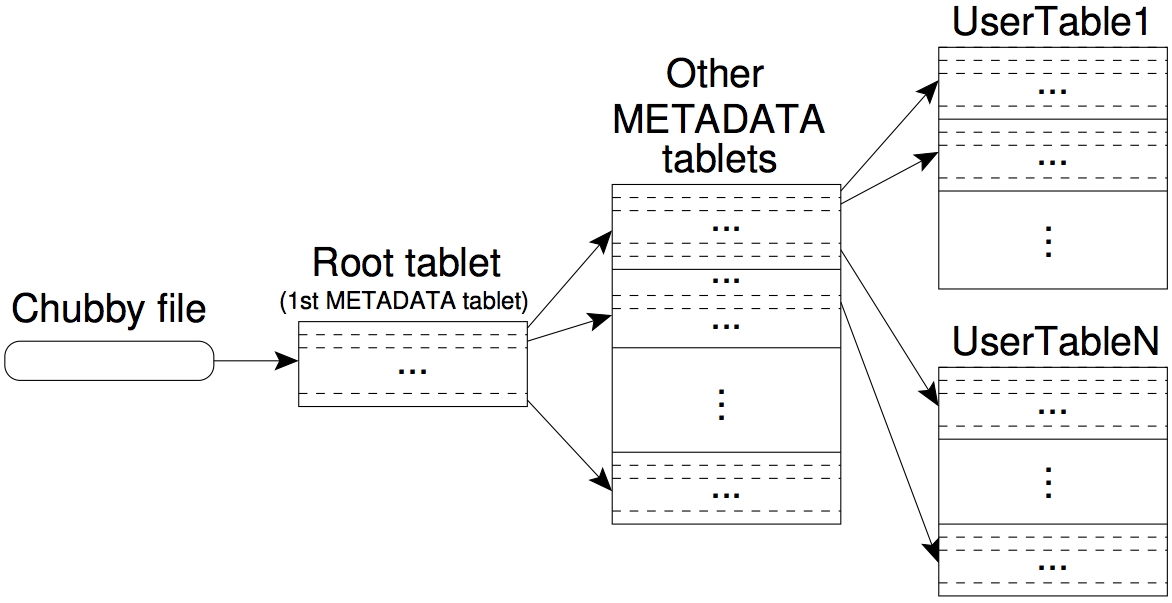
\includegraphics[width=0.48\textwidth]{tablet}
        \caption{\small Tablet location hierarchy.}
        \label{fig02}
\end{figure}


 첫번째 단계는 Chubby에 저장된 루트 타블렛(\textit{root tablet})의 위치를 가지고 있는 파일이다. 루트 타블렛은 특별한 METADATA 테이블에 모든 타블렛들의 위치를 가지고 있다. 각각의 METADATA 타블렛은 유저 타블렛들의 집합에 대한 위치를 가지고 있다. 루트 타블렛은 단지 METADATA 테이블의 첫번째 타블렛에 불과하지만, 타블렛 위치 계층구조가 3단계 이상을 가지지 않게하기 위해 특별하게 취급된다. 루트 타블렛은 절대 쪼개지지 않는다.

METADATA 테이블은 타블렛의 테이블 식별자와 마지막 row를 인코딩한 row key 아래에 타블렛 위치를 저장한다. 각각의 METADATA row 는 메모리에 있는 데이터의 대략 1KB를 저장한다. 그다지 크지 않은 128MB METADATA 타블렛 사이즈로, 우리의 3단계 계층구조의 위치 스키마는 $2^{34}$ 타블렛들의 어드레스를 하는 것이 가능하다(또는 128MB 타블렛에서 $2^{61}$ 바이트).

클라이언트 라이브러리는 타블렛 위치를 캐쉬한다. 만약 클라이언트가 타블렛의 위치를 모르거나, 캐쉬된 위치정보가 잘못되었다는 것을 발견하면 타블렛 계층구조를 타고 위로 올라가게 된다. 만약 클라이언트의 캐쉬가 비어있으면, 위치 알고리즘은 Chubby로 부터 읽어오는 것을 포함하여 네트워크를 3번 왕복하는 것을 요구한다. 만약 캐쉬의 정보가 오래되었다면, 위치 알고리즘은 네트워크를 여섯번 왕복하도록 만든다. 왜냐하면, METADATA 타블렛들이 빈번하게 움직이지 않는다는 가정하에, 빠뜨렸던 것을 발견할 수 있기 때문이다.  타블렛 위치가 메모리에 저장되기 때문에 구글파일시스템(GFS)에 접근할 필요가 없긴 하지만, 앞으로는 클라이언트 라이브러리가 타블렛 위치들을 미리 패치하도록 함으로써 이러한 비용을 점점 줄여나갈 것이다 : 메타데이타 테이블을 읽을때는 반드시 하나 이상 타블렛의 메타데이터를 읽는다.

우리는 메타데이터 테이블의 각 타블렛에서 발생하는 모든 이벤트 로그와 같은 2차 정보들을 저장한다. 이러한 정보는 디버깅이나 성능을 분석하는데 매우 유용하다.
 
\subsection{Tablet Assignment}
타블렛들은 각각 하나의 타블렛 서버에 할당된다. 마스터는 살아있는 타블렛 서버들을 확인하고, 타블렛 서버에 할당되어진 타블렛들이 현재 수행하는 작업을 추적하고, 작업이 할당되지 않은 타블렛 또한 확인한다. 태블릿이 할당되지 않고, 태블릿을 위해 충부한 여유공간을 가진 태블릿 서버가 있는 경우, 마스터는 태블릿 로드 요청을 전송함으로써, 태블릿을 할당한다. 

빅 테이블은 태블릿 서버를 추적하기 위해 춰비(Chubby)를 사용한다. 태블릿 서버가 시작하면, Chubby를 생성하고, 특정 Chubby 디렉토리내의 고유한 이름을 가진 파일에 배타적인 락(exclusive lock)을 획득한다. 마스터는 태블릿 서버를 탐색하기 위해 서버 디렉토리를 모니터링한다.
태블릿 서버는 Chubby 세션 끝남에 따라 서버에서 야기한 네트워크 파티션 등으로 인해 배타적 락을 잃게되면 해당 태블릿 서비스를 중단한다.
Chubby는 네트워크 트래픽을 발생시키지 않고도 태블릿 서버에게 락을 가지고 있는지를 체크할 수 있도록 효율적인 메카니즘을 제공한다.
태블릿 서버는 파일이 존재하는 한 파일에 대한 배타적인 락을 재 획득하려고 시도할 것이다. 만약 파일이 더이상 존재하지 않으면,  태블릿 서버는 스스로 종료(kill)하고 태블릿 서버를 제공하지 않게 된다.
태블릿 서버가 종료될 때마다, 마스터가 좀더 빠르게 태블릿을 재할당할 수 있도록, 태블릿 서버는 자신이 가지고 있던 락을 해제(release)한다.
마스터는 태블릿 서버가 더이상 태블릿을 제공하지 않는지 감지하고 가능한한 빨리 다른 태블릿들을 재할당하는 역할을 수행한다.
태블릿 서버가 태블릿을 더이상 제공하지 않는 지를 감지하기 위해, 마스터는 주기적으로 태블릿이 가진 락의 상태에 대해 태블릿 서버에게 물어본다.
만약에 태블릿 서버가 락을 잃어버렸다고 보고하거나, 마스터가 태블릿 서버에게 여러번 시도해도 요청이 도달하지 않는 경우,
마스터는 서버의 파일에 대한 배타적인 락에 대한 획득을 시도한다.
마스터가 락을 획득할 수 있으면, 처비는 살아있고 태블릿 서버는 죽었거나 처비에 도달하는 데 문제가 가지고 있다는 것이므로,
마스터는 서버 파일을 삭제함으로써 태블릿 서버가 더이상 서비스를 제공할 수 없음을 보장한다.
한번 서버 파일이 삭제되면, 마스터는 이전에 서버에 지정된 모든 태블릿을 미지정 태블릿 셋으로 이동시킬 수 있다.
빅테이블 클러스터는 마스터와 취비 사이의 네트워크 문제들에 취약하지 않음을 보장하기 위해, 취비 세션이 만료되면 마스터가 스스로 마스터 자신을 종료한다.
하지만, 앞에서 언급한 바와 같이, 마스터 실패는 태블릿 서버 태블릿들의 할당을 변경하지 않는다.

마스터가 클러스터 관리시스템에 의해 시작될 때, 마스터는 태블릿들의 할당을 변경하기 전에 현재 할당된 것들을 탐색할 필요가 있다.
마스터는 시작 시 다음과 같은 단계를 실행한다.
\be
\ii 마스터는 동시에 마스터가 인스턴스화(instantiations)되는 것을 막기 위해, Chubby내에 있는 고유한 마스터 락을 건다.
\ii 마스터는 살아있는 서버들을 찾기 위해 Chubby내에 있는 서버 디렉토리를 스캔한다.
\ii 마스터는 어떤 태블릿들이 이미 각 서버에 할당되었는지 탐색하기 위해 모든 살아있는 태블릿 서버와 통신한다.
\ii 마스터는 태블릿 집합을 이해(learn)할 수 있는 메타데이터(METADATA) 테이블을 스캔한다.
\ee
마스터의 스캔 도중에 이미 할당되지 않은 태블릿을 만날 때마다,
마스터는 태블릿 할당의 자격이 있는 태블릿을, 할당되지 않는 태블릿의 집합에 해당 태블릿을 추가한다.

한가지 복잡한 문제는 METADATA 태블릿들이 할당되기 전까지는 METADATA 테이블에 대한 스캔이 일어나지 않는다는 점이다.
따라서, 4단계의 스캔을 시작하기 전에, 만약 3단계 수행동안에 루트 태블릿에 대한 할당을 찾지 못했다면, 마스터는 할당되지 않은 태블릿 집합으로 해당 루트 태블릿을 추가한다. 여기서 루트 태블릿을 추가하는 작업은 루트 태블릿이 할당될 것이라는 점을 보장한다.
루트 태블릿이 모든 METADATA 태블릿들의 네임을 포함하고 있기 때문에, 마스터는 루트 태블릿 스캔을 완료하면, 모든 태블릿에 대한 내용을 파악하게 된다.

기존 태블릿 집합은 테이블이 생성되거나 삭제될 때만 변경이 일어나며,
두 개의 기존 태블릿들은 하나의 큰 태블릿으로 만들기 위해 합쳐지거나, 기존 태블릿은 두 개의 작은 태블릿으로 분할되기도 한다.
마스터는 모든 태블릿들을 시작하기 때문에 이러한 변경사항을 추적할 수 있다.
태블릿 분할은  태블릿 서버에 의해 시작되기 때문에 특별하게 취급된다.
태블릿 서버는 METADATA 테이블내에 있는 새로운 태블릿에 대한 정보를 기록함으로써 분할 작업을 커밋(commit)한다.
분할 작업이 커밋되면, 태블릿 서버는 마스터에게 이를 통보한다.
태블릿 서버가 죽거나 마스터가 죽어서 분할 통보가 유실되는 경우,
지금 분할을 마친 태블릿을 로드하기 위해 태블릿 서버에게 요청할 때, 마스터는 새로운 태블릿을 감지한다.
태블릿 서버가 METADATA 테이블내에서 찾은 태블릿 항목은 마스터가 로드를 위해 요청한 태블릿의 일부만을 지정하기 때문에, 
태블릿 서버는 분할을 마스터에게 통보할 것이다.


\subsection{Tablet Serving}

빅테이블내 태블릿에 대한 상세한 저장소 표현은 그림 \ref{fig:sstable}와 같다.
빅테이블에서 주요한 저장단위는 SSTable이다. SSTable은 구글 인프라스트럭쳐에서도 사용되는 파일 포맷이다. 
SSTable은 임의의 스트링으로된 키와 밸류를 매핑하는 정렬되어 있고 변경할 수 없는 맵이다. 
주어진 키와 연관된 밸류를 효과적으로 읽을 수 있고 주어진 키 범위내에 속한 밸류의 집합에 대해 반복하며  읽을 수 있는 연산을 제공하고 있다.
SSTable의 인덱스는 SSTable의 끝부분에 저장되어 있으며, SSTable을 엑세스할 때 메모리에서 읽어온다. 
다시 말해, 주어진 엔트리를 디스크를 한번만 읽어는 것 만으로 읽어올 수 있다는 의미다. 
전체 SSTable 엔트리를 메인 메모리에 필요에 따라 저장할 수도 있다.

\begin{figure}[htb]
        \centering
        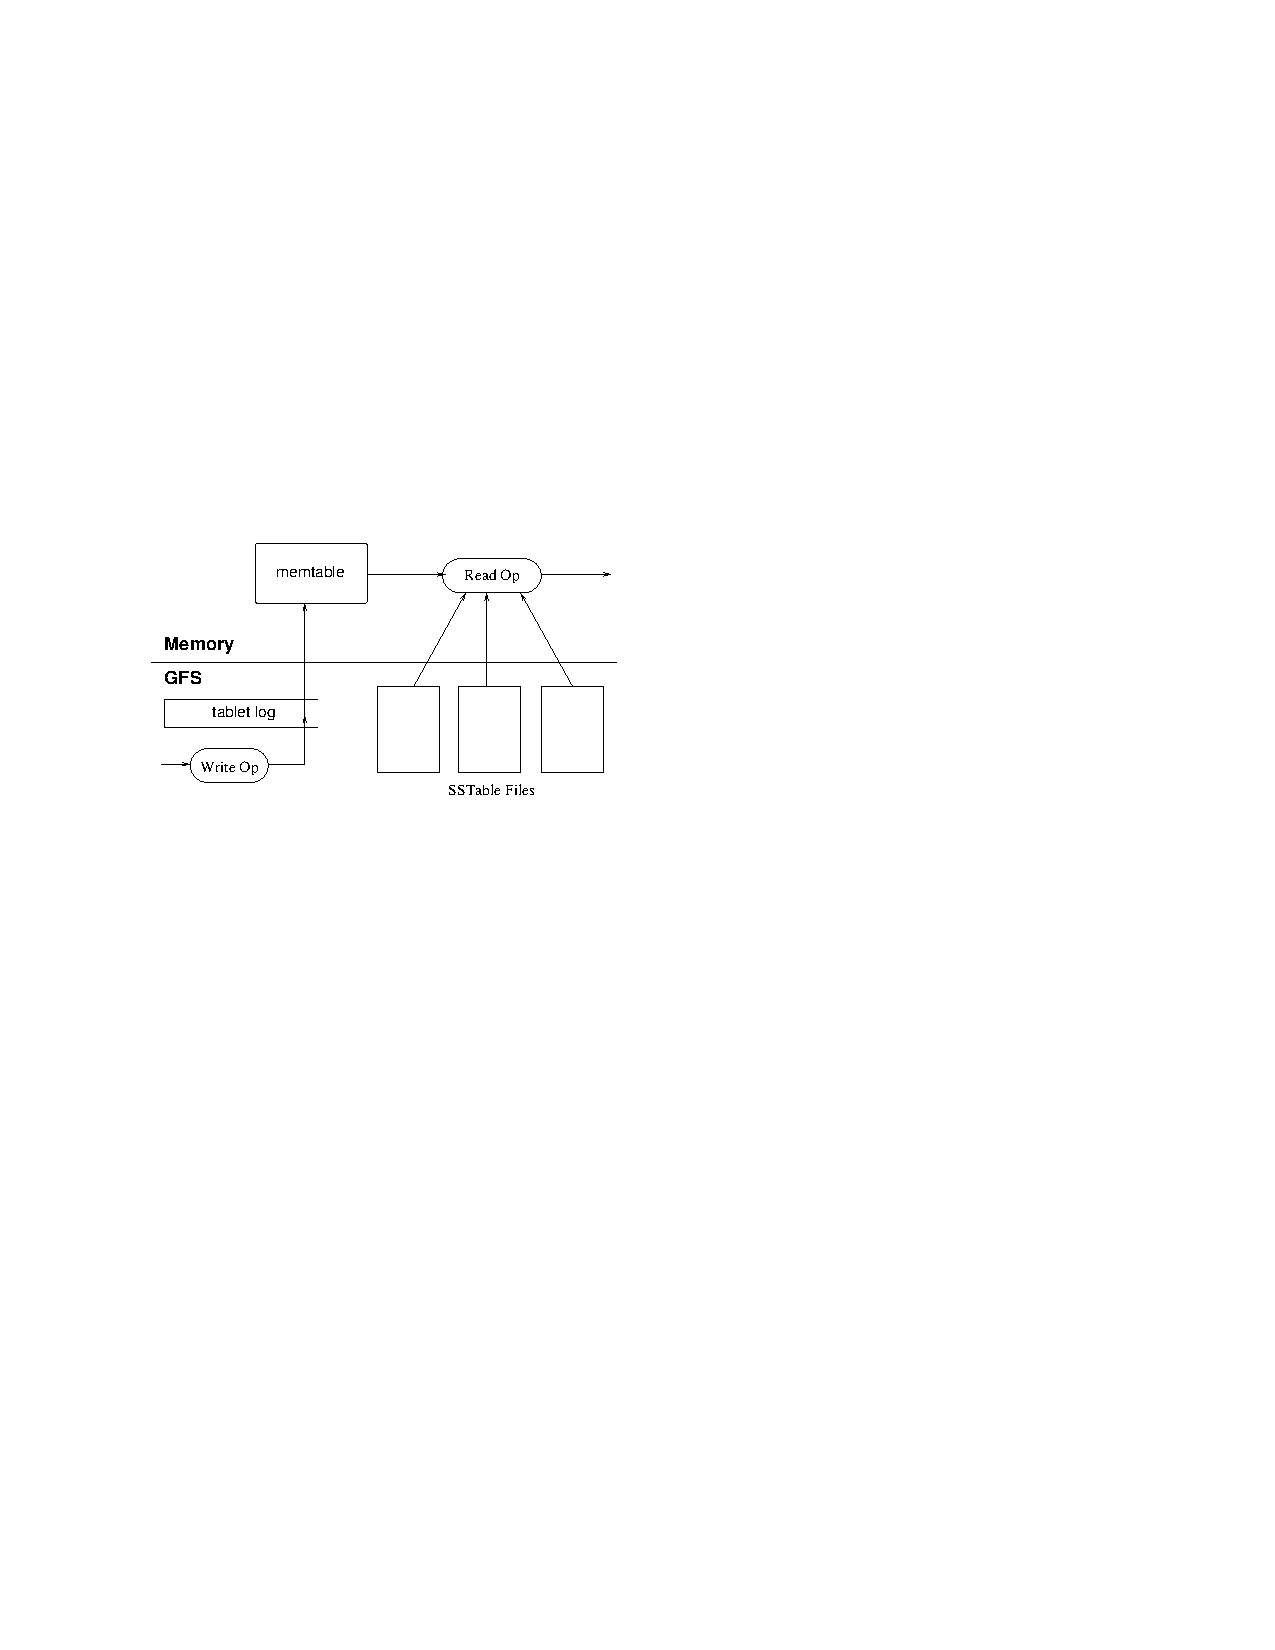
\includegraphics[width=0.48\textwidth]{sstable}
        \caption{    태블릿 표현}
        \label{fig:sstable}
\end{figure}

주어진 태블릿은 많은 SSTable들로 표현된다. 뮤테이션(mutation)을 직접 수행하기보다 복구(recovery)를 지원하기 위해 로그에 먼저 쓰기를 커밋한다. 이러한 로그 엔트리는 메인 메모리내의 memtable을 통해 쓴다. 따라서, SSTable은 태블릿 상태에 대한 스냅샷과 같은 역할을 한다. 
실패시, 가장 최근 스냅샷이후의 최근 로그 엔트리를 이용하여 복구가 이루어진다.



\section{Conclusion}
본 기술문서에서 HBase나 카산드라(Cassandra)와 같은 칼럼 패밀리 데이터베이스들의 선조격인 빅테이블에 대해 살펴봤다.
구글의 빅테이블은 초창기부터 많은 영향을 끼친 NoSQL 데이터베이스 중 하나였다. 이름을 보면 표 구조가 떠오르지만, 실제로는 희박한 칼럼으로 되어 있고 스키마는 없다. 이걸 테이블 구조로 생각하는 것은 도움이 되지 않는다. 그보다는 두 단계로 된 맵으로 생각하는 편이 낫다.
구조야 어떻든, 빅 테이블은 HBase나 카산드라(Cassandra) 같은 이후에 나온 데이터베이스에 영향을 주었다.

빅테이블 형식의 데이터 모델을 가진 데이터베이스는 흔히 칼럼 저장소라 부르지만, 이 이름은 다른 녀석을 나타내는 용어였다. 
C-스토어(C-Store) 같은 NoSQL 이전의 칼럼 저장소는 SQL과 관계형 모델에도 잘 맞았다. 다른 점은 데이터의 물리적 저장 방식이였다.
대다수 데이터베이스는 행을 저장 단위로 다뤄 쓰기 성능에 도움을 준다. 그러나 쓰기는 거의 없지만 많은 행에 대해 칼럼 몇 개만 한꺼번에 읽어야 하는 경우도 있다. 이런 경우라면, 모든 행에 대한 칼럼 그룹을 저장 단위로 사용하는 편이 낫다. 이런 이유로 이런 데이터베이스를 칼럼 저장소라 부른 것이다.

빅테이블과 그 후손은 칼럼 그룹(칼럼 패밀리)을 함께 저장한다는 개념을 따랐지만, 관계형 모델과 SQL을 버렸다는 점에서 C-스코어나 그 친구들과는 다르다. 

%When a write operation arrives at a tablet server, the server checks that it is well-formed, and that the sender is authorized to perform the mutation. Authorization is performed by reading the list of permitted writers from a Chubby file (which is almost always a hit in the Chubby client cache). A valid mutation is written to the commit log. Group commit is used to improve the throughput of lots of small mutations [13, 16]. After the write has been committed, its contents are inserted into the memtable.
%When a read operation arrives at a tablet server, it is similarly checked for well-formedness and proper authorization. A valid read operation is executed on a merged view of the sequence of SSTables and the memtable. Since the SSTables and the memtable are lexicographically sorted data structures, the merged view can be formed efficiently.
%Incoming read and write operations can continue while tablets are split and merged.
%
%\subsection{Compactions}
%As write operations execute, the size of the memtable increases. When the memtable size reaches a threshold, the memtable is frozen, a new memtable is created, and the frozen memtable is converted to an SSTable and written to GFS. This minor compaction process has two goals: it shrinks the memory usage of the tablet server, and it reduces the amount of data that has to be read from the commit log during recovery if this server dies. Incoming read and write operations can continue while compactions occur.
%Every minor compaction creates a new SSTable. If this behavior continued unchecked, read operations might need to merge updates from an arbitrary number of SSTables. Instead, we bound the number of such files by periodically executing a merging compaction in the background. A merging compaction reads the contents of a few SSTables and the memtable, and writes out a new SSTable. The input SSTables and memtable can be discarded as soon as the compaction has finished.
%A merging compaction that rewrites all SSTables into exactly one SSTable is called a major compaction. SSTables produced by non-major compactions can contain special deletion entries that suppress deleted data in older SSTables that are still live. A major compaction, on the other hand, produces an SSTable that contains no deletion information or deleted data. Bigtable cycles through all of its tablets and regularly applies major compactions to them. These major compactions allow Bigtable to reclaim resources used by deleted data, and also allow it to ensure that deleted data disappears from the system in a timely fashion, which is important for services that store sensitive data.
%
%
%Refinements
%The implementation described in the previous section required a number of refinements to achieve the high performance, availability, and reliability required by our users. This section describes portions of the implementa- tion in more detail in order to highlight these refinements.
%Locality groups
%Clients can group multiple column families together into a locality group. A separate SSTable is generated for each locality group in each tablet. Segregating column families that are not typically accessed together into sep- arate locality groups enables more efficient reads. For example, page metadata in Webtable (such as language and checksums) can be in one locality group, and the contents of the page can be in a different group: an ap-plication that wants to read the metadata does not need to read through all of the page contents.
%In addition, some useful tuning parameters can be specified on a per-locality group basis. For example, a lo- cality group can be declared to be in-memory. SSTables for in-memory locality groups are loaded lazily into the memory of the tablet server. Once loaded, column fam- ilies that belong to such locality groups can be read without accessing the disk. This feature is useful for small pieces of data that are accessed frequently: we use it internally for the location column family in the METADATA table.
%Compression
%Clients can control whether or not the SSTables for a locality group are compressed, and if so, which com- pression format is used. The user-specified compres- sion format is applied to each SSTable block (whose size is controllable via a locality group specific tuning pa- rameter). Although we lose some space by compress- ing each block separately, we benefit in that small por- tions of an SSTable can be read without decompress- ing the entire file. Many clients use a two-pass custom compression scheme. The first pass uses Bentley and McIlroy’s scheme [6], which compresses long common strings across a large window. The second pass uses a fast compression algorithm that looks for repetitions in a small 16 KB window of the data. Both compression passes are very fast—they encode at 100–200 MB/s, and decode at 400–1000 MB/s on modern machines.
%Even though we emphasized speed instead of space re- duction when choosing our compression algorithms, this two-pass compression scheme does surprisingly well. For example, in Webtable, we use this compression scheme to store Web page contents. In one experiment, we stored a large number of documents in a compressed locality group. For the purposes of the experiment, we limited ourselves to one version of each document in- stead of storing all versions available to us. The scheme achieved a 10-to-1 reduction in space. This is much better than typical Gzip reductions of 3-to-1 or 4-to-1 on HTML pages because of the way Webtable rows are laid out: all pages from a single host are stored close to each other. This allows the Bentley-McIlroy algo- rithm to identify large amounts of shared boilerplate in pages from the same host. Many applications, not just Webtable, choose their row names so that similar data ends up clustered, and therefore achieve very good com- pression ratios. Compression ratios get even better when we store multiple versions of the same value in Bigtable.
%Caching for read performance
%To improve read performance, tablet servers use two lev- els of caching. The Scan Cache is a higher-level cache that caches the key-value pairs returned by the SSTable interface to the tablet server code. The Block Cache is a lower-level cache that caches SSTables blocks that were read from GFS. The Scan Cache is most useful for appli- cations that tend to read the same data repeatedly. The Block Cache is useful for applications that tend to read data that is close to the data they recently read (e.g., se- quential reads, or random reads of different columns in the same locality group within a hot row).
%Bloom filters
%As described in Section 5.3, a read operation has to read from all SSTables that make up the state of a tablet. If these SSTables are not in memory, we may end up doing many disk accesses. We reduce the number of accesses by allowing clients to specify that Bloom fil- ters [7] should be created for SSTables in a particu- lar locality group. A Bloom filter allows us to ask whether an SSTable might contain any data for a spec- ified row/column pair. For certain applications, a small amount of tablet server memory used for storing Bloom filters drastically reduces the number of disk seeks re- quired for read operations. Our use of Bloom filters also implies that most lookups for non-existent rows or columns do not need to touch disk.
%Commit-log implementation
%If we kept the commit log for each tablet in a separate log file, a very large number of files would be written concurrently in GFS. Depending on the underlying file system implementation on each GFS server, these writes could cause a large number of disk seeks to write to the different physical log files. In addition, having separate log files per tablet also reduces the effectiveness of the group commit optimization, since groups would tend to be smaller. To fix these issues, we append mutations to a single commit log per tablet server, co-mingling mutations for different tablets in the same physical log file [18, 20].
%Using one log provides significant performance ben- efits during normal operation, but it complicates recov- ery. When a tablet server dies, the tablets that it served will be moved to a large number of other tablet servers: each server typically loads a small number of the orig- inal server’s tablets. To recover the state for a tablet, the new tablet server needs to reapply the mutations for that tablet from the commit log written by the original tablet server. However, the mutations for these tablets were co-mingled in the same physical log file. One ap- proach would be for each new tablet server to read this full commit log file and apply just the entries needed for the tablets it needs to recover. However, under such a scheme, if 100 machines were each assigned a single tablet from a failed tablet server, then the log file would be read 100 times (once by each server).
%We avoid duplicating log reads by first sort- ing the commit log entries in order of the keys ⟨table, row name, log sequence number⟩. In the sorted output, all mutations for a particular tablet are contiguous and can therefore be read efficiently with one disk seek followed by a sequential read. To parallelize the sorting, we partition the log file into 64 MB seg- ments, and sort each segment in parallel on different tablet servers. This sorting process is coordinated by the master and is initiated when a tablet server indicates that it needs to recover mutations from some commit log file.
%Writing commit logs to GFS sometimes causes perfor- mance hiccups for a variety of reasons (e.g., a GFS server machine involved in the write crashes, or the network paths traversed to reach the particular set of three GFS servers is suffering network congestion, or is heavily loaded). To protect mutations from GFS latency spikes, each tablet server actually has two log writing threads, each writing to its own log file; only one of these two threads is actively in use at a time. If writes to the ac- tive log file are performing poorly, the log file writing is switched to the other thread, and mutations that are in the commit log queue are written by the newly active log writing thread. Log entries contain sequence numbers to allow the recovery process to elide duplicated entries resulting from this log switching process.
%Speeding up tablet recovery
%If the master moves a tablet from one tablet server to another, the source tablet server first does a minor com- paction on that tablet. This compaction reduces recov- ery time by reducing the amount of uncompacted state in the tablet server’s commit log. After finishing this com- paction, the tablet server stops serving the tablet. Before it actually unloads the tablet, the tablet server does an- other (usually very fast) minor compaction to eliminate any remaining uncompacted state in the tablet server’s log that arrived while the first minor compaction was being performed. After this second minor compaction is complete, the tablet can be loaded on another tablet server without requiring any recovery of log entries.
%Exploiting immutability
%Besides the SSTable caches, various other parts of the Bigtable system have been simplified by the fact that all
%of the SSTables that we generate are immutable. For ex- ample, we do not need any synchronization of accesses to the file system when reading from SSTables. As a re- sult, concurrency control over rows can be implemented very efficiently. The only mutable data structure that is accessed by both reads and writes is the memtable. To re- duce contention during reads of the memtable, we make each memtable row copy-on-write and allow reads and writes to proceed in parallel.
%Since SSTables are immutable, the problem of perma- nently removing deleted data is transformed to garbage collecting obsolete SSTables. Each tablet’s SSTables are registered in the METADATA table. The master removes obsolete SSTables as a mark-and-sweep garbage collec- tion [25] over the set of SSTables, where the METADATA table contains the set of roots.
%Finally, the immutability of SSTables enables us to split tablets quickly. Instead of generating a new set of SSTables for each child tablet, we let the child tablets share the SSTables of the parent tablet.






\bibliographystyle{abbrv}
\bibliography{sqlonhadoop}

\end{document}
